\usetikzlibrary{shapes}
\begin{problem}{Search: Multiple Choice and Short Answer Questions}

\begin{question}[12]
Consider the following true/false questions with each question worth 2 points. For the following search problems, assume every action has a cost of at least $\epsilon$, with $\epsilon > 0$.  Assume any heuristics used are consistent. 

\vspace{2mm}
\hspace{0.5mm}
Depth-first tree-search on a finite graph is guaranteed to be complete. \\
\solution{\emptycircle}{\FourAATrue} \textbf{True}
\hspace{5mm}
\solution{\emptycircle}{\FourAAFalse} \textbf{False} \\
\solution{}{\FourAAReason}

\vspace{2mm}
\hspace{0.5mm}
Breadth-first tree-search on a finite graph is guaranteed to be complete. \\
\solution{\emptycircle}{\FourABTrue} \textbf{True}
\hspace{5mm}
\solution{\emptycircle}{\FourABFalse} \textbf{False} \\
\solution{}{\FourABReason}

\vspace{2mm}
\hspace{0.5mm}
Iterative deepening tree-search on a finite graph is guaranteed to be complete. \\
\solution{\emptycircle}{\FourACTrue} \textbf{True}
\hspace{5mm}
\solution{\emptycircle}{\FourACFalse} \textbf{False} \\
\solution{}{\FourACReason}

\vspace{2mm}
\hspace{0.5mm}
For all graphs without cycles, graph-search contains a larger frontier than tree-search. \\
\solution{\emptycircle}{\FourADTrue} \textbf{True}
\hspace{5mm}
\solution{\emptycircle}{\FourADFalse} \textbf{False} \\
\solution{}{\FourADReason}

\vspace{2mm}
\hspace{0.5mm}
Iterative deepening graph-search has the time complexity of BFS and the space complexity of DFS. \\
\solution{\emptycircle}{\FourAETrue} \textbf{True}
\hspace{5mm}
\solution{\emptycircle}{\FourAEFalse} \textbf{False} \\
\solution{}{\FourAEReason}

\vspace{2mm}
\hspace{0.5mm}
If $h_{1}$(s) is a consistent heuristic and $h_{2}$(s) is a consistent heuristic, then min($h_{1}$(s), $h_{2}$(s)) must be consistent. \\
\solution{\emptycircle}{\FourAFTrue} \textbf{True}
\hspace{5mm}
\solution{\emptycircle}{\FourAFFalse} \textbf{False} \\
\solution{}{\FourAFReason}
\end{question} 
\vspace{2mm}

\begin{question}[5] 
Consider the state space graph shown below. S is the start state and G is the goal state. The costs for each edge are shown on the graph. For the following table below, fill in potential heuristic values such that the heuristic is admissible but not consistent. 

\vspace{10mm}
\begin{centering} 
\hspace{10mm}
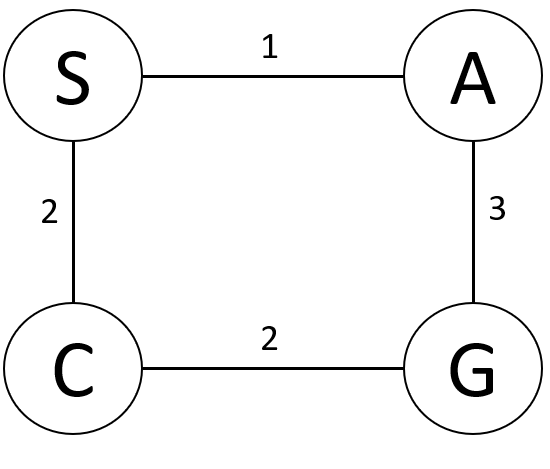
\includegraphics[scale=.6]{figures/Consistent.png} 
\hspace{32mm}{\raisebox{32mm}{
\begin{tabular}{ |p{1.8cm}|p{1.2cm}|  }
\hline
\multicolumn{2}{|c|}{\textbf{Heuristic Function}} \\
\hline
\textbf{State} & \textbf{$h(s)$}  \\
\hline
$S$ & \solution{}{\FourBS}  \\
\hline
$A$ & \solution{}{\FourBA}  \\
\hline
$C$ & \solution{}{\FourBC}   \\
\hline
$G$ &  0 \\
\hline
\end{tabular}}}
\end{centering}

\solution{}{\FourBReason}

\end{question}

\end{problem}